\documentclass{acm_proc_article-sp}
\usepackage{amsmath}
\usepackage{algorithm}
\usepackage{algpseudocode}
\usepackage{fancyvrb}

\begin{document}
\title{Verifying Nonlinear Elementary Functions in the Embedded GNU C Library}

\maketitle
\begin{abstract}
We present a novel approach solve the probabilistic bounded reachability problem of 
hybrid systems with parameter uncertainty. Standard approaches to this problem require 
numerical solutions for large optimization problems, and become unfeasible for systems 
involving nonlinear dynamics over the reals. Our approach combines randomized 
sampling of probabilistic system parameters, SMT-based bounded reachability analysis, 
and statistical tests. We utilize $\delta-$complete decision procedures 
to solve reachability analysis in a sound way, i.e., we always decide correctly if, for a given
combination of parameters, the system actually reaches the unsafe region.
Compared to standard simulation-based analysis methods, our approach supports 
non-deterministic branching, increases the coverage of simulation, and avoids the
zero-crossing problem. We demonstrate that our method is feasible for general
hybrid systems with parametric uncertainty by applying the implemented tool {\bf SReach} to
a range of nonlinear hybrid systems with parametric uncertainty.

\hide{
We present a novel approach that combines Satisfiability Modulo Theories (SMT) and 
statistical testing to solve the probabilistic bounded reachability problem of 
hybrid systems with parameter uncertainty. That is, we want to find out whether 
a hybrid system with probabilistic system parameters reaches an unsafe region of the
state space within a finite number of steps with a probability greater (or less) than a 
fixed threshold. Standard approaches to this problem require numerical solutions for 
large optimization problems, and become unfeasible for systems involving nonlinear dynamics
over the reals. Our approach solves the reachability problem by combining randomized 
sampling of probabilistic system parameters, SMT-based bounded reachability analysis, 
and statistical tests. In particular, we utilize $\delta-$complete decision procedures 
to solve reachability analysis in a sound way, i.e., we always decide correctly if, for a given
combination of parameters, the system actually reaches the unsafe region (in the opposite case 
we may generate false positives, but this can be controlled by a precision parameter $\delta>0$).
Compared to other simulation-based analysis methods, our approach supports 
non-deterministic branching, increases the coverage of simulation, and avoids the
zero-crossing problem. We demonstrate that our method is feasible for general
hybrid systems with parametric uncertainty by applying the implemented tool {\bf SReach} to
a wide range of nonlinear hybrid systems.}
%to two representative examples - the prostate cancer treatment control and the cardiac system, 
%and further through applications to additional benchmarks.
\vspace{-.7cm}
\end{abstract}

%\category{H.4}{Information Systems Applications}{Miscellaneous}
%\category{D.2.8}{Software Engineering}{Metrics}[complexity measures, performance measures]
%\terms{Theory}
%\keywords{ACM proceedings, \LaTeX, text tagging}

\section{Introduction}\label{sec:intro}

% Need a paragrapgh or two to explain why the tool is interesting and
% significant should be provided.

\dReach{} is a bounded reachability analysis tool for hybrid systems.
It encodes bounded reachability problems of hybrid systems as
first-order formulas over the real numbers, and solves them using
$\delta$-decision procedures in the SMT solver
\dReal{}~\cite{DBLP:conf/cade/GaoKC13}. \dReach{} is able to handle a
wide range of highly nonlinear hybrid systems~\cite{CMSB14,DBLP:conf/fmcad/GaoKC13,DBLP:conf/hybrid/KapinskiDSA14,6868816}.
Figure~\ref{fig:prostate-example} highlights some of its features: on
the left is an example of some nonlinear dynamics that \dReach{} can
handle, and on the right a visualized counterexample generated by
\dReach{} on this model.
\begin{figure}[!h]
  \subfloat[An example of nonlinear hybrid system model: off-treatment
  mode of the prostate cancer treatment model~\cite{CMSB14}\label{subfig-1:prostate}]{
    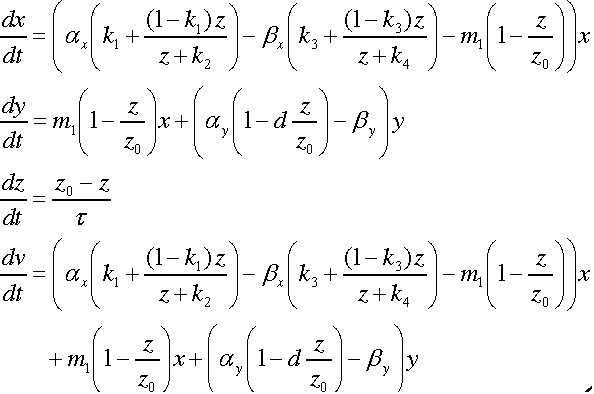
\includegraphics[width=0.45\textwidth]{images/prostatebw-mode2.pdf}
  }
  \hfill
  \subfloat[Visualization of a generated counterexample. Change in the shade of colors represents discrete mode changes.]{%
    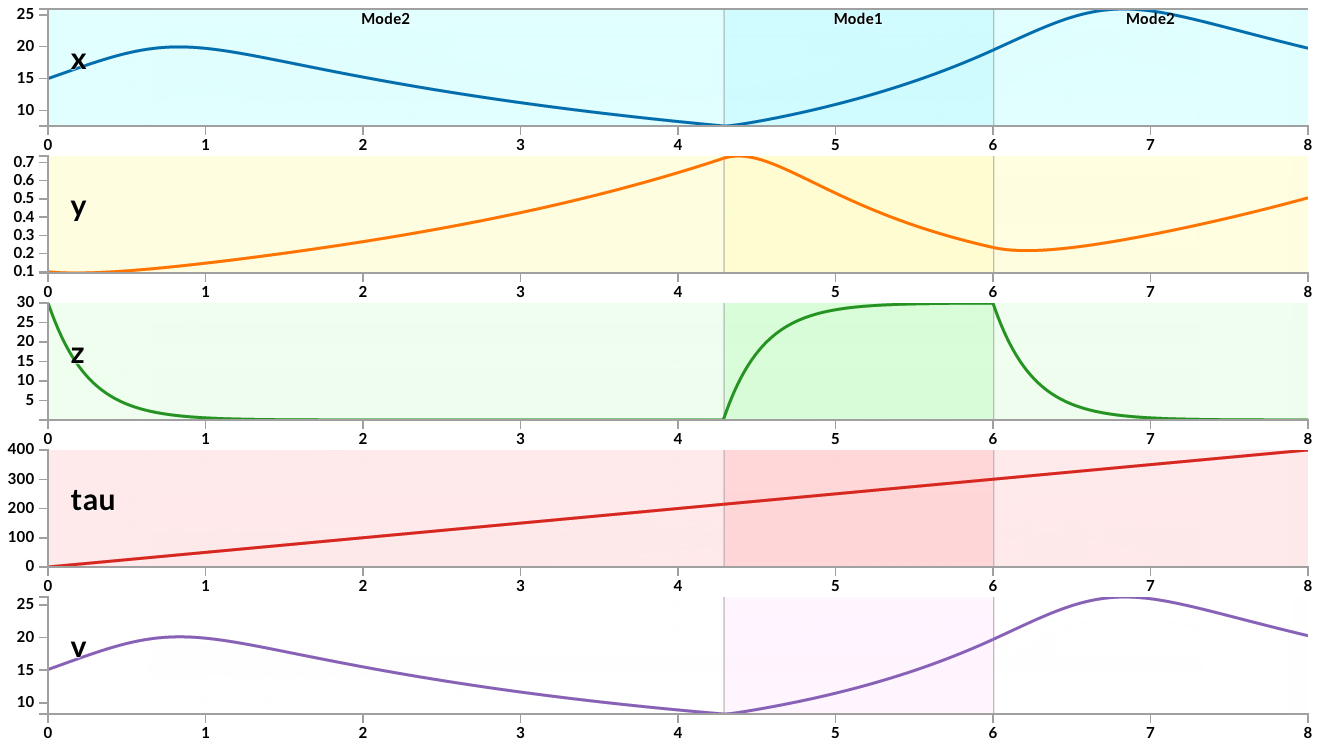
\includegraphics[width=0.48\textwidth]{images/prostate}
  }
  \caption{An example of nonlinear dynamics and counterexample-generation.}
  \label{fig:prostate-example}
\end{figure}

It is well-known that the standard bounded reachability problems for
simple hybrid systems are already highly
undecidable~\cite{DBLP:conf/hybrid/AlurCHH92}.
Instead, we work in the framework of $\delta$-reachability of hybrid systems~\cite{DBLP:journals/corr/GaoKCC14}.
Here $\delta$ is an arbitrary positive rational number, provided by the user to
specify the bound on numerical errors that can be tolerated in the analysis.
For a hybrid system $H$ and an unsafe region $\unsafe$ (both encoded as logic formulas),
the $\delta$-reachability problem asks for one of the following answers:
\begin{itemize}
        \item {\sf safe}: $H$ cannot reach $\unsafe$.
        \item {\sf $\delta$-unsafe}: $H^{\delta}$ can reach $\unsafe^{\delta}$.
\end{itemize}
Here, $H^{\delta}$ and $\unsafe^{\delta}$ encode ($\delta$-bounded) overapproximations
of $H$ and $\unsafe$, defined explicitly as their syntactic variants.%(See Section~\ref{sec:delta-reachability} in the Appendix.)
It is important to note that the definition makes the answers no weaker than standard reachability:
When {\sf safe} is the answer, we know for certain that $H$ does not reach
the unsafe region (no $\delta$ is involved); when {\sf $\delta$-unsafe} is the answer,
we know that there exists some $\delta$-bounded perturbation of the system that can render it unsafe.
Since $\delta$ can be chosen to be very small, {\sf$\delta$-unsafe} answers in fact
discover robustness problem in the system, which should be regarded as unsafe indeed.
We have proved that bounded $\delta$-reachabilty is decidable for a wide range
of nonlinear hybrid systems, even with reasonable complexity bounds~\cite{DBLP:journals/corr/GaoKCC14}.
This framework provides the formal correctness guarantees of \dReach{}.

Apart from solving $\delta$-reachability, the following key features of \dReach{}
distinguish it from other existing tools in this
domain~\cite{DBLP:journals/jlp/FranzleTE10,DBLP:conf/cav/FrehseGDCRLRGDM11,DBLP:journals/tac/AlthoffK14,DBLP:conf/hybrid/Frehse05,DBLP:conf/icons/HerdeEFT08,DBLP:conf/rtss/ChenAS12,DBLP:conf/aaai/CimattiMT12}.
%insert explanations for each item.
\begin{enumerate}
\item Expressiveness. \dReach{} allows the user to describe hybrid
  systems using first-order logic formulas over real numbers with a
  wide range of nonlinear functions. This allows the user to specify
  the continuous flows using highly nonlinear differential equations,
  and the jump and reset conditions with complex Boolean combinations
  of nonlinear constraints. \dReach{} also faithfully translates mode
  invariants into $\exists\forall$ logic formulas, which can be
  directly solved under certain restrictions on the invariants.
\item Property-guided search. \dReach{} maintains logical encodings
  (the same approach as~\cite{DBLP:conf/aaai/CimattiMT12}), whose size
  is linear in the size of the inputs, of the reachable states of a
  hybrid system~\cite{DBLP:journals/corr/GaoKCC14}. The tool searches
  for concrete counterexamples to falsify the reachability properties,
  instead of overapproximating the full reachable states. This avoids
  the usual state explosion problem in reachable set computation,
  because the full set of states does not need to be explicitly
  stored. This change is analogous to the difference between SAT-based
  model checking and BDD-based symbolic model checking.
\item Tight integration of symbolic reasoning and numerical solving.
  \dReach{} delegates the reasoning on discrete mode changes to SAT
  solvers, and uses numerical constraint solving to handle nonlinear
  dynamics. As a result, it can combine the full power of both
  symbolic reasoning and numerical analysis algorithms. In particular,
  all existing tools for reachable set computation can be easily
  plugged-in as engines for solving the continuous part of the
  dynamics, while logic reasoning tools can overcome the difficulty in
  handling complex mode transitions.
\end{enumerate}
The paper is structured as follows. We describe the system architecture in Section 2,
and give some details about the logical encoding in the tool in Section 3.
We then explain the input format and usage in Section 4. %More details and examples are given in the Appendix.

%Realistic hybrid systems involves nonlinear ODEs with transcendental
%functions. \dReach{} allows users to specify a hybrid system in a
%nonlinear signature as it is without linearizing or overapproximating
%it. Users can provide the tool with a numerical error bound $\delta$,
%a bounded time horizon $[0, T]$, and a maximum number of mode switches
%$k$ for the analysis. As a result of analysis, \dReach{} will return
%either \textbf{$\delta$-sat} with a concrete counterexample, or
%\textbf{unsat} which does not involve numerical errors. We also
%provide a visualization for the $\delta$-sat case to help
%understand the analysis result.

% TODO: Need to differentiate this paper from FMCAD paper
%  - FMCAD: underlying solving techniques for SMT with ODEs
%  - TACAS: tool, encoding, using solver...

%%% Local Variables:
%%% mode: latex
%%% TeX-master: "main"
%%% End:


\section{Preliminaries}

We give an overview of the floating point implementation of the sine function in the Embedded GNU C Library. We then briefly review SMT solving of nonlinear formulas over the reals and features of our solver dReal~\cite{}.

\subsection{Floating-Point Representations and Errors}

Floating point representations. 

It is well-known that floating point computation introduces errors. For basic arithmetic operations, the error can be estimated by the following formula. 

We use this formula to overapproximate the result of floating point arithmetic with real arithmetic. 

\subsection{Structure of Continuous Programs}

main issue: bounded or unbounded loops. 

The basic idea of evaluating the sine function is, naturally, to combine the periodic nature of the function and estimate the value with Taylor series. For each input number, the routine checks its position with respect to multiples of $\pi/4$, and then evaluate the value with appropriate Taylor expansion. 

The implementation of the sine function has the following structure. 
\begin{verbatim}
Give a simplified skeleton
\end{verbatim}

We should highlight the bit-level operations and table look up in the formula. 

\subsection{SMT over the Reals}


SMT formulas over the real numbers are very hard to solve when nonlinear functions are involved. 
We let $\mathcal{F}$ denote a set of continuous real functions. $\mathcal{L}_{\mathcal{F}}$ denotes the first-order signature and $\mathbb{R}_{\mathcal{F}}$ is the standard structure $\langle \mathbb{R}, \mathcal{F}\rangle$. We can then consider the SMT problem over $\mathbb{R}_{\mathcal{F}}$, namely, satisfiability of quantifier-free $\mathcal{L}_{\mathcal{F}}$-formulas over $\mathbb{R}_{\mathcal{F}}$. We consider formulas whose variables take values from bounded intervals. Because of this, it is more convenient to directly write the bounds on existential quantifiers and express bounded SMT problems as $\Sigma_1$-sentences with bounded quantifiers.
\begin{definition}[Bounded $\Sigma_1$-Sentences]
A bounded $\Sigma_1$-sentence in $\mathcal{L}_{F}$ is
$$\varphi:\ \exists^{I_1}x_1\cdots \exists^{I_n}x_n. \psi(x_1,...,x_n).$$
We can write a bounded $\Sigma_1$-sentence as $\exists^{\vec I}\vec x.\psi(\vec x)$ for short.
\end{definition}
It is well-known that the first-order theory with transcendental functions is undecidable. However, it is recently shown in~\cite{} that if we consider numerical perturbations as part of the decisions of the logic formulas, we have a decidable problem~\cite{}. Let $\delta$ be any positive rational number. Define a syntactic variation of a formula as follows:
\begin{definition}[$\delta$-Weakening~\cite{DBLP:conf/cade/GaoAC12}]
Let $\delta\in \mathbb{Q}^+\cup\{0\}$ be a constant and $\varphi$ be a
$\Sigma_1$-sentence in a standard form 
$$\varphi:= \exists^{\vec I}\vec
x\;(\bigwedge_{i=1}^m (\bigvee_{j=1}^{k_i}
f_{ij}(\vec x)= 0)).$$The $\delta$-weakening of $\varphi$ defined as:
$$\varphi^{\delta}:= \exists^{\vec I} \vec x\;(\bigwedge_{i=1}^m(\bigvee_{j=1}^k
|f_{ij}(\vec x)|\leq \delta)).$$
\end{definition}
The $\delta$-decision problem is then defined as follows. On a given SMT formula $\varphi$, we can ask for one of the following answers:
\begin{itemize}
 \item {\sf unsat}: $\varphi$ is unsatisfiable.
 \item {\sf $\delta$-sat}: $\varphi^{\delta}$ is satisfiable.
\end{itemize}
When the two cases overlap, either answer can be returned. It is important to note that error is only one-sided. 

With such relaxation, $\delta$-complete decision procedures can fully exploit the power of scalable numerical algorithms to solve nonlinear problems, and at the same time provide suitable correctness guarantees for many correctness-critical problems. {\sf dReal}\footnote{{\sf dReal} is available at \url{http://dreal.cs.cmu.edu}.} implements this framework. It solves SMT problems over the reals with nonlinear functions, such as polynomials, sine, exponentiation, logarithm, etc. The user can obtain certificates (proof of unsatisfiability or solution) for the answers.

%%% Local Variables:
%%% mode: latex
%%% TeX-master: "main"
%%% End:


\section{The Test-and-Infer Loop}

Testing is an incomplete method of checking specifications of a
function. It samples points from the domain of a function and checks
whether properties hold at those points or not. Sampling larger number
of points may give higher confidence on the correctness of a function.
However, it is practically infeasible to sample all the points in the
domain even if the domain is bounded and this remains testing
incomplete. For example, there are more than $10^{18}$ double-precision
floating-point numbers between $0.0$ and $1.0$. In a modern computer,
it takes more than a second to test an implementation of sine function
on $10^9$ points. It means that it takes more than 30 years to give a
complete coverage on the implementation for the interval $[0.0, 1.0]$.

Test-and-infer is an approach to enhance this weakness of testing.
Whenever it samples a point $c$ from the domain and test a property,
it infers a neighbor $I = [c - \delta, c + \delta]$ of the point $c$
which shares the same test result at point $c$. Using the technique,
we can efficiently cover a region of a domain by testing a point and
it accelerates the overall verification process. In our experiment
shows that it takes about XXX minutes to check a property of sine
implementation on the same interval $[0, 1]$.

\subsection{The Main Algorithm}
We want to partition a given subset $S \subseteq \mathbb{R}$ of the
domain of a nonlinear elementary function $f : \mathbb{R} \to
\mathbb{R}$ into two sets of intervals:
\begin{align*}
  P & = \{ [l, u] \mid \forall x \in [l, u]. \; | F_f(x) - f(x) | \le \varepsilon \}\\
  F & = \{ [l, u] \mid \forall x \in [l, u]. \; | F_f(x) - f(x) | > \varepsilon \}
\end{align*}
where $F_f$ denotes the function encoding the program. The set $P$
represents a set of points which satisfy the specification while the
set $F$ represents all points which possibly violate the
specification.

\begin{algorithm}
  \centering
  \caption{Test-and-Infer}
  \label{fig:test-and-infer}
  \begin{algorithmic}[1]
    \Procedure{Test-and-Infer}{f, g, lb, ub, $\varepsilon$}
        \State $c \gets lb$
        \State $P \gets \{\}$
        \State $F \gets \{\}$
        \While{$c \le ub$}
            \If {$ |f(c) - g(c)| \le \varepsilon$}
                % Good
                \State $\delta \gets \mathrm{FindDelta}(f, g(c), c, \varepsilon)$
                \State $P \gets P \cup
                                \{ [c - \delta, c + \delta] \}$
            \Else
                % Bad
                \State $\delta \gets \mathrm{FindDelta}(f, g(c), c, \varepsilon)$
                \State $F \gets F \cup
                                \{ [c - \delta, c + \delta] \}$
            \EndIf
            \State $c \gets c + \delta$
        \EndWhile
    \EndProcedure
  \end{algorithmic}
\end{algorithm}

Figure~\ref{fig:test-and-infer} illustrates the main algorithm of our
approach. Given a function $f$, range $[lb, ub]$, and an error-bound
$\varepsilon$, \texttt{Test-and-Infer} returns the two sets $P$ and
$F$. After initialization (line 2 - 4), it executes $f(c)$ and store
the result at $r$ (line 6).

\subsection{Encoding the Implementation}






Show many snippets of the code. 





\subsection{Verifying Good Intervals}
For each good input $a\in \mathbb{R}$ and error bound $\varepsilon$,
we find a neighborhood $I$ around $a$ such that
$$\forall x\in I.\; |F_{\sin}(x)-\sin(x)|\leq \varepsilon$$
where $F_{\sin}$ denotes the function encoding the program.

By triangle inequality, we have
\begin{eqnarray}
|F_{\sin}(x) - \sin(x)| \leq |F_{\sin}(x) - \sin(a)| + |\sin(x) - \sin(a)|,
\end{eqnarray}
and we only need to show

\begin{eqnarray}
\forall x\in I.\; |F_{\sin}(x) - \sin(a)| + |\sin(x) - \sin(a)| \leq \varepsilon.
\end{eqnarray}

For this, we can check satisfiability of the negation of the formula, i.e.:
\begin{eqnarray}
\exists x\in I.\; |F_{\sin}(x) - \sin(a)| + |\sin(x) - \sin(a)| > \varepsilon.
\end{eqnarray}

With Taylor expansion, we know
\begin{eqnarray}
|\sin(x) - \sin(a)| > \cos(a) |x - a| - \frac{\sin(a)}{2}(x-a)^2 + ... %check it
\end{eqnarray}

Thus, we only need to show
\begin{eqnarray}
\exists x\in I.\; |F_{\sin}(x) - \sin(a)| + \cos(a) |x - a| -
\frac{\sin(a)}{2}(x-a)^2 > \varepsilon.
\end{eqnarray}

The program encoding can be sliced based on monitoring on the input.
Basically we only need the slice that's used in producing the output.

\subsection{Debugging Bad Intervals}

For a bad input $b$ and error bound $\varepsilon$, we aim to find a
neighborhood $I$ around $b$ such that the error always exhibits:

$$ \forall x\in I.\; |F_{\sin}(x) - \sin(x)| > \varepsilon$$

The bad cases usually come from some bugs in the program. For that we
can have a formula encoding conditions on intermediate variables.
Formalize this ...

%%% Local Variables:
%%% mode: latex
%%% TeX-master: "main"
%%% End:


\section{Case Study}
% PZ: I think the two sentences below should in 'Methods' section.
%We have developed an open-source tool dReach using OCaml to perform $\delta$-complete reachability 
%analysis for hybrid systems \cite{dreach}. dReach is built upon our SMT solver dReal \citep{dreal} 
%that implements a $\delta$-complete decision procedure. 

To exemplify different aspects of our parameter synthesis framework, we carried out a case study on
a model of the electrical dynamics of cardiac cells. All the experiments reported below were done 
using a machine with two Intel Xeon E5-2650 2.00GHz processors and 64GB RAM. The precision $\delta$
was set to $0.001$.

\begin{figure}[t]
\centering
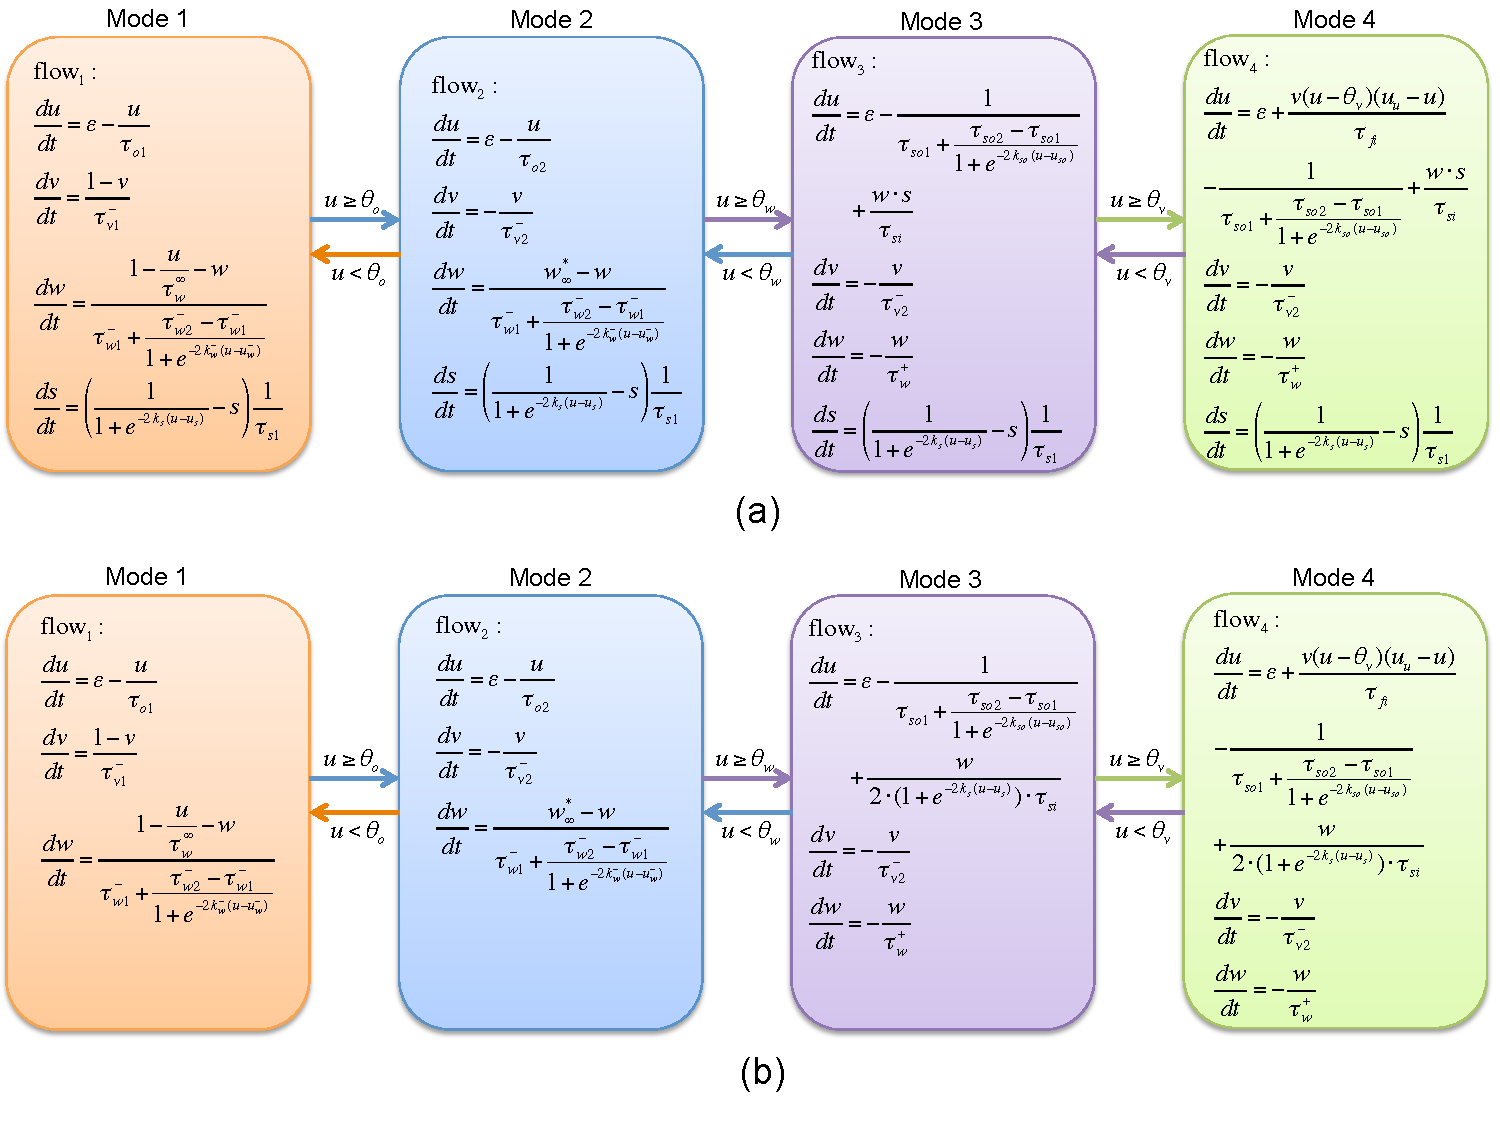
\includegraphics[scale=0.5]{fig-cardiac-new}
\caption{Hybrid models of cardiac cells. (a) BCF model. (b) FK model.}
\label{model}
 %\vspace{-0.7cm}
\end{figure}

\subsection{Hybrid models of cardiac cells}
The heart rhythm is enabled by the electrical activity of cardiac muscle cells, which make up the atria and ventricles. The electrical dynamics of cardiac cells is governed by the organized opening and closing of ion channel gates on the cell membrane. Improper functioning of the cardiac cell ionic channels can cause the cells to lose excitability, which disorders electric wave propagation and leads to cardiac abnormalities such as ventricular \textit{tachycardia} or \textit{fibrillation}. Hybrid automata models have been developed recently in order to understand the mechanisms of cardiac disorders, including the Fenton-Karma (FK) model \cite{fenton98} and the Bueno-Cherry-Fenton (BCF) model \cite{orovio08}. 

\paragraph{BCF Model.} 
In this model, the change of cells transmembrane potential $u$, in response to an external stimulus $\epsilon$ from neighboring cells, is regulated by a fast ion channel gate $v$ and two slow gates $w$ and $s$.
Figure \ref{model}(a) shows the four modes associated with the BCF model. In Mode $1$, gates $v$ and $w$ are open and gate $s$ is closed. The transmembrane potassium current causes the decay of $u$. The cell is resting and waiting for stimulation. We assume an external stimulus $\epsilon$ equals to $1$ which lasts for $1$ millisecond. The stimulation causes $u$ to increase, which may trigger $\jump_{1 \rightarrow 2}: u \geq \theta_o$. When this jump takes place, the system switches to Mode 2 and $v$ starts closing, and the decay rate of $u$ changes. The system will jump to Mode 3 if $u \geq \theta_w$. In Mode 3, $w$ is also closing; $u$ is governed by the potassium current and the calcium current. When $u \geq \theta_v$, Mode 4 can be reached, which signals a successful action potential (AP) initiation. In Mode 4, $u$ reaches its peak due to the fast opening of the sodium channel. The cardiac muscle contracts and $u$ starts decreasing. 

\paragraph{FK Model.} 
As shown in Figure \ref{model}(b), this model comprises the same four modes and equations of the BCF model, except that the current change induced by gate $s$ is reduced to an explicit term which is integrated
in the right-hand side of $du/dt$. Similarly to the BCF model, an AP can be successfully initiated when Mode 4 is reached. 

We specified both the BCF and the FK model using dReach's modeling language. Starting from the state ($u = 0$, $v = 1$, $w = 1$, $s = 0$) in Mode 1, we checked whether Mode 4 is reachable using the parameter values presented in \cite{orovio08}. This was true (\ie, dReach returned $\delta$-$\mathsf{sat}$) for both models. 
The simulation of a few witness trajectories are shown in Figure \ref{trace} (the stimulus $\epsilon$ was reset every $500$ milliseconds).


\begin{figure}[thb]
\centering
\subfigure[]{
  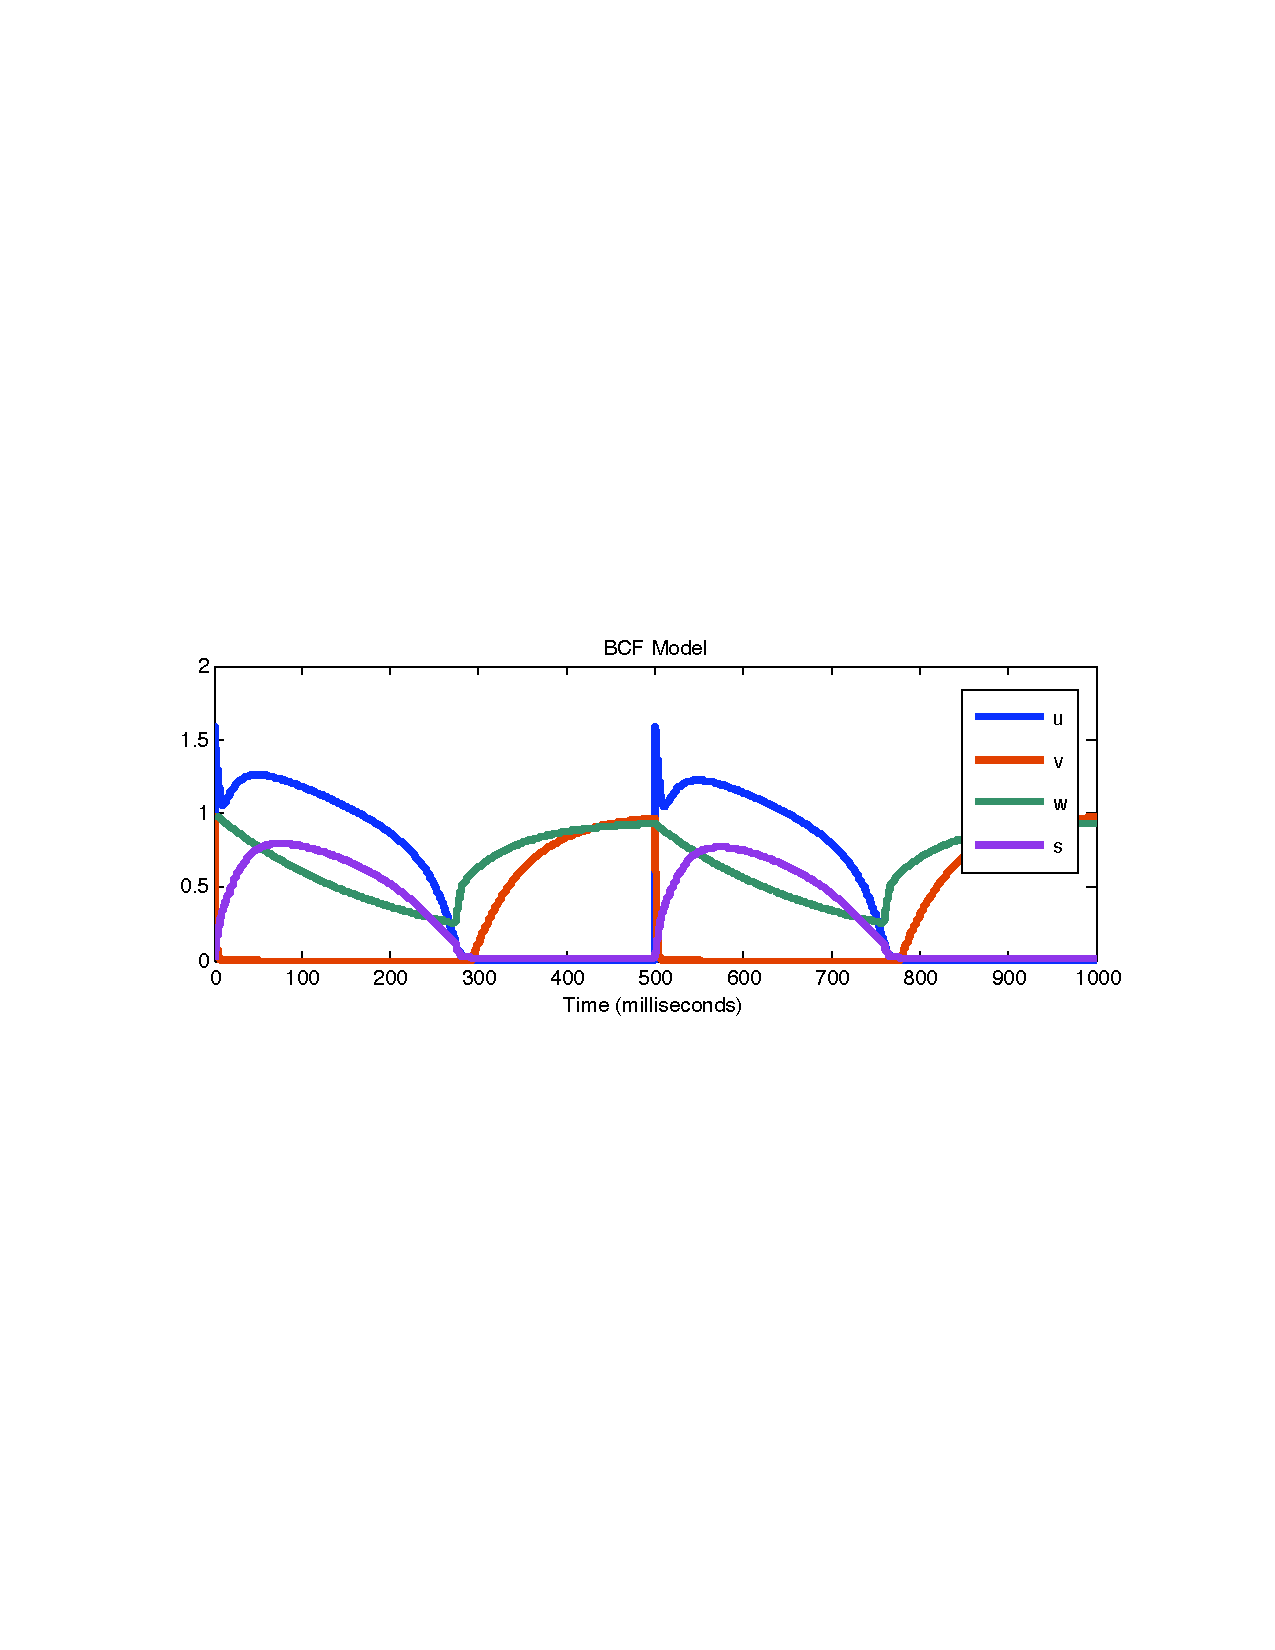
\includegraphics[width=8cm]{fig-bcf}
} 
\subfigure[]{
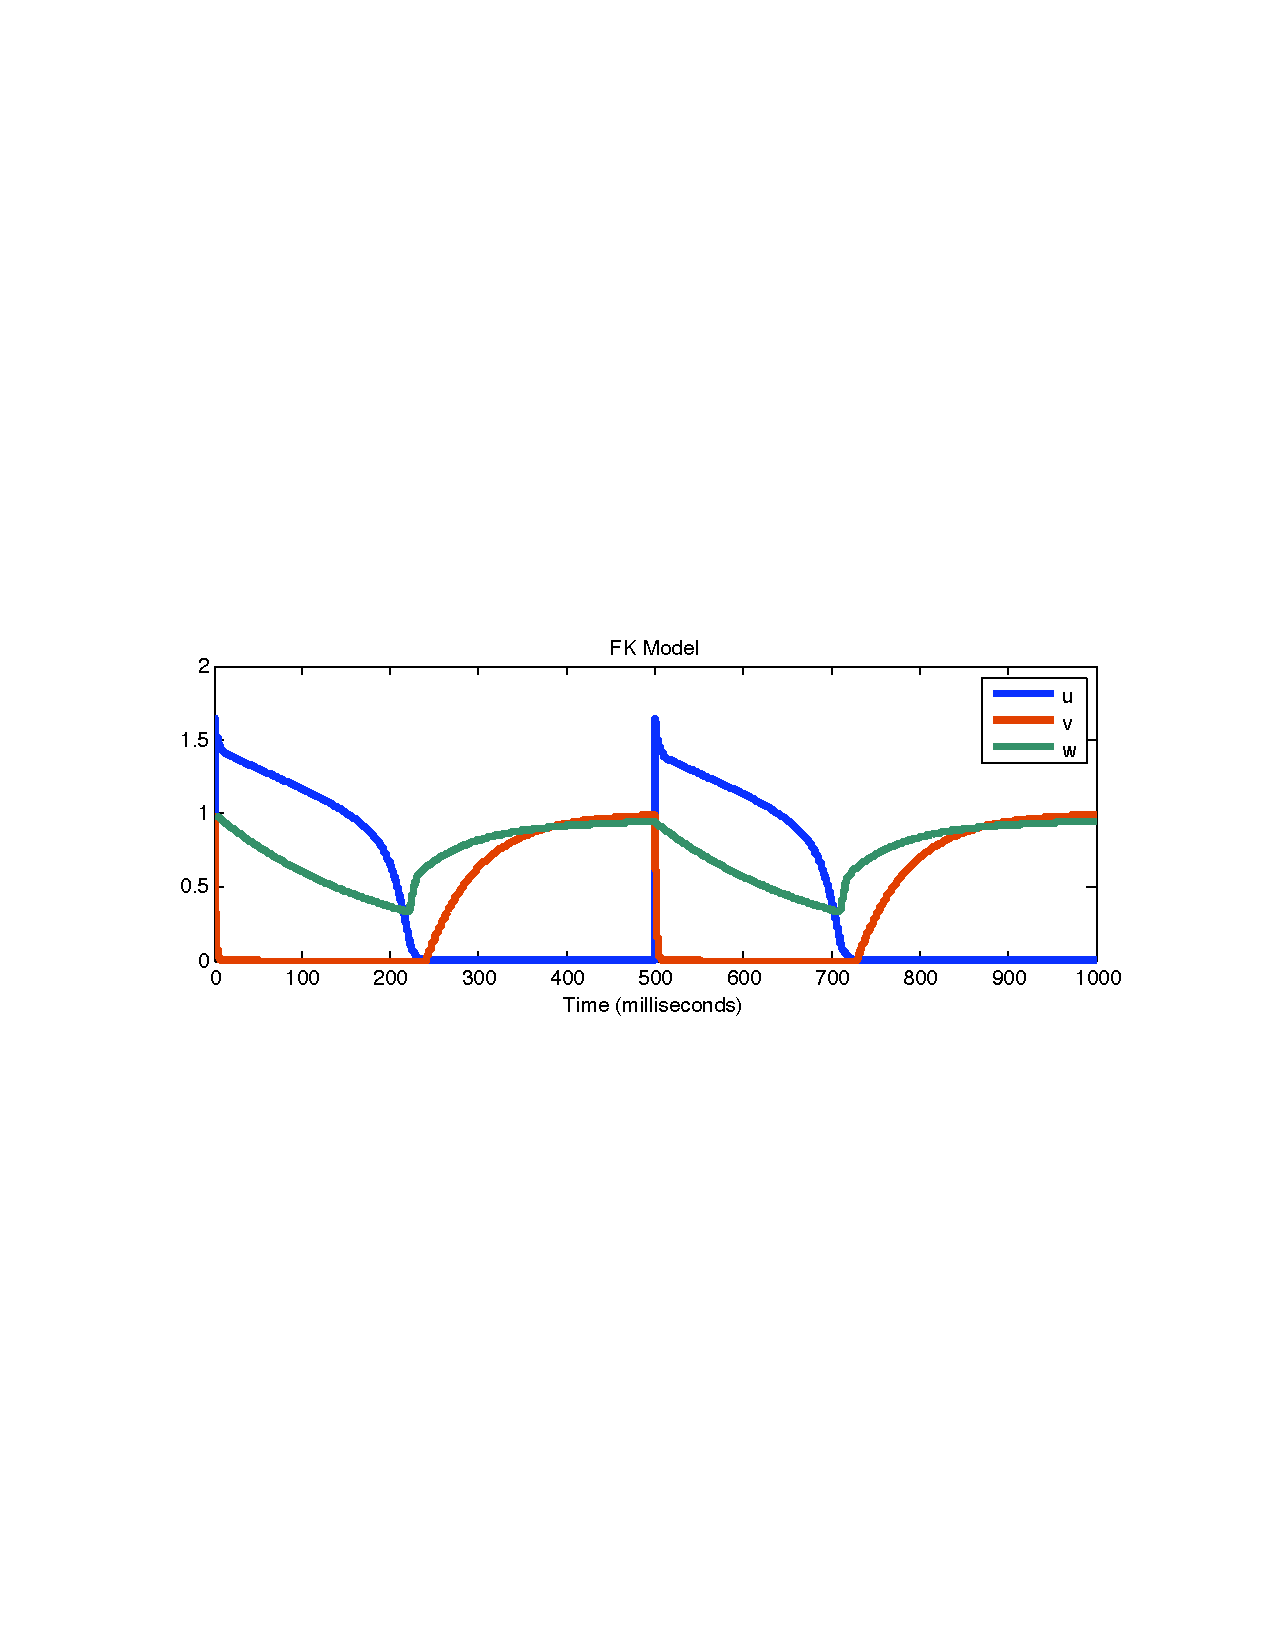
\includegraphics[width=8cm]{fig-fk}
}
\caption{The simulated time profile of BCF and FK.}
\label{trace}
 %\vspace{-0.7cm}
\end{figure}


\subsection{Model falsification}
Both the BCF and FK models were able to reproduce essential characteristics (\eg, steady-state action potential duration) observed in human ventricular cells \cite{fenton98,orovio08}. However, ventricular cells comprise three cell types, which possess different dynamical characteristics. For instance, Figure \ref{ap} shows that time courses of APs for epicardial and endocardial human ventricular cells have different morphologies \cite{nabauer96}. An important \textit{spike-and-dome} AP morphology can only be observed in epicardial cells but not endocardial cells. Hence, in a model-based study, one needs to identify cell-type-specific parameters to take account into cellular heterogeneity. The feasibility of this task will depend on the model of choice, as certain model would be impossible to reproduce a dynamical behavior no matter which parameter values are used. Here we illustrate that such models can be ruled out efficiently using our $\delta$-decision based parameter synthesis framework.

\paragraph{Robustness.} 
To ensure proper functioning of cardiac cells in noisy environments, an important property of the system is to filter out insignificant stimulation. Thus, we expected to see that APs could not be initiated for small $\epsilon$. Starting from the state ($u = 0$, $v = 1$, $w = 1$, $s = 0$, $\epsilon \in [0.0,0.25]$) in Mode 1, we checked the reachability of Mode 4. The $\mathsf{unsat}$ answer was returned by dReach for both the BCF and FK
model, showing that the models are robust to stimulation amplitude.

\begin{figure}[th]
\centering
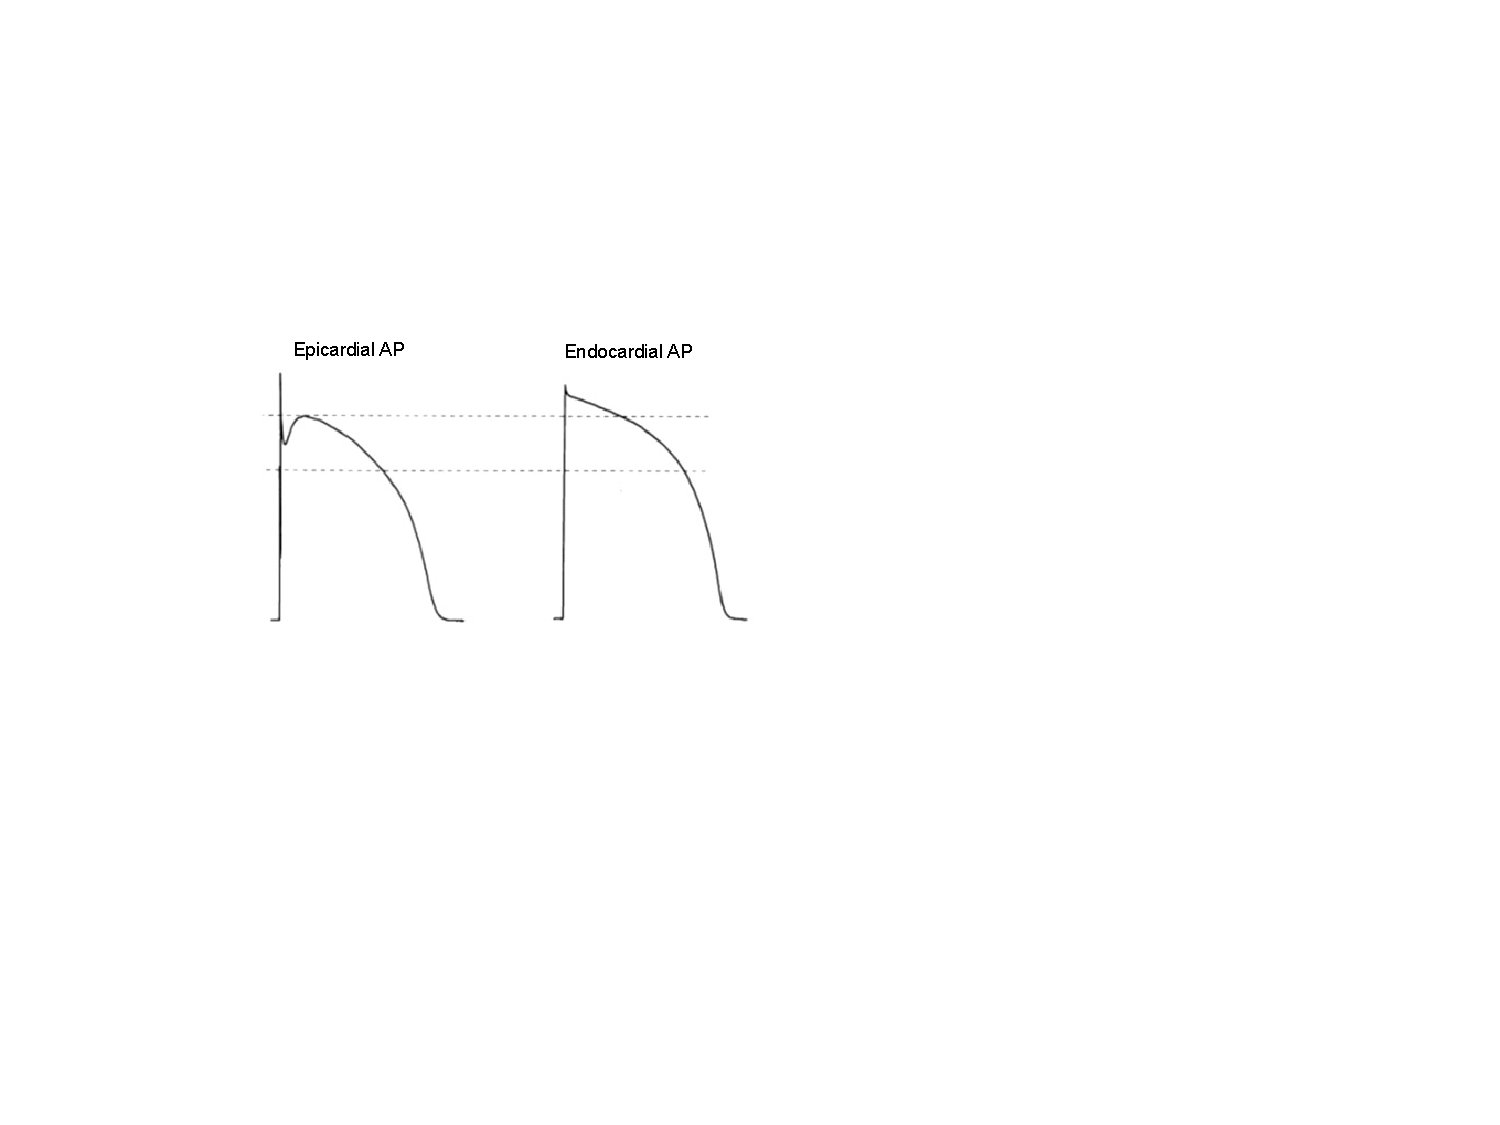
\includegraphics[scale=0.8]{fig-ap}
\caption{Experimental AP morphology \cite{nabauer96}.}
\label{ap}
 %\vspace{-0.7cm}
\end{figure}

\paragraph{AP morphology.}
Next we tested whether the models can reproduce the spike-and-dome AP morphology of epicardial cells. We introduced two auxiliary modes (Mode 5 and 6). The system will jump from Mode 4 to Mode 5 if $\tau \le 10$, and will jump from Mode 5 to Mode 6 if $\tau \le 30$. In Modes 5 and 6, we enforced invariants $1.0 \le u \le 1.15$ and $1.18 \le u \le 2.0$, respectively, to depict the spike-and-dome morphology observed experimentally \cite{nabauer96}. We then checked reachability of Mode 6, starting from Mode 1 in state ($u = 0$, $v = 1$, $w = 1$, $s = 0$, $\epsilon \in [0.9,1.1]$, $\tau_{si} \in [1,2]$, $u_s \in [0.5,2]$). The $\delta$-$\mathsf{sat}$ answer
was returned for BCF, while $\mathsf{unsat}$ was returned for FK, indicating that the FK model cannot reproduce spike-and-dome shapes using reasonable parameter values. Hence, FK is not suitable to study the dynamics of epicardial cells.

We remark that any $\mathsf{unsat}$ answer is guaranteed to be correct. This effectively
means that we proved that the FK model cannot reach Mode 6 for {\em any} starting state in the 
rectangle ($u = 0$, $v = 1$, $w = 1$, $s = 0$, $\epsilon \in [0.9,1.1]$, $\tau_{si} \in [1,2]$, 
$u_s \in [0.5,2]$). Sampling-based approaches cannot have the same level of certainty, while other
approaches cannot handle the complexity of the flows in the model.


\subsection{Parameter identification for cardiac disorders}

When the system cannot reach Mode 4, the cardiac cell loses excitability, which might lead to tachycardia or fibrillation. Starting with Mode 1, our next goal was to identify parameter ranges for which the system will never go into Mode 4. In what follows, we focused our study on the BCF model. 
Grosu {\em et al.}~\cite{grosu11} have tackled this parameter identification problem by linearizing the BCF model into a piecewise-multiaffine system (referred as MHA). With this simplification, parameter ranges could be identified using the Rovergene tool \cite{rovergene}. However, the BCF and MHA models have different sets of parameters. Here we aimed at identifying disease-related ranges of the original BCF parameters. It can be derived from the model equations that $\tau_{o1}$ and $\tau_{o2}$ govern the dynamics of $u$ in Mode 1 and Mode 2 respectively, and hence determine whether $\jump_{1\rightarrow 2}$ and  $\jump_{2\rightarrow 3}$ can be triggered. For $\tau_{o1}$, we performed a binary search in value domain $[0.0001,0.01]$ to obtain a threshold value $\theta_{o1}$ such that Mode 4 is unreachable if $\tau_{o1} \in (0, \theta_{o1})$ while Mode 4 is reachable if $\tau_{o1} =  \theta_{to1}$. Specifically, for each candidate value $\theta^i_{o1}$, we checked the reachability of Mode 4 with the initial state ($u = 0$, $v = 1$, $w = 1$, $s = 0$, $\theta_{o1} = \theta^i_{o1}$). We set the next candidate to be $(\theta^i_{o1} -\theta_{l})/2$ if $\mathsf{sat}$ was returned, or $(\theta_{r} - \theta^i_{o1})/2$ if $\mathsf{unsat}$ was returned, where $\theta_{l}$ is the largest $\mathsf{unsat}$ candidate and $\theta_{r}$ is the smallest $\mathsf{sat}$ candidate. 

In this manner, we identified $\theta_{o1}$ to be $0.006$, which suggest that when $\tau_{o1} \in (0, 0.006)$, the system will always stay in Mode 1. Similarly, we also obtained a threshold value of $0.13$ for $\tau_{o2}$, such that Mode 3 cannot be reached when $\tau_{o2} \in (0, 0.13)$. Furthermore, whether the system can jump from Mode 3 to Mode 4 depends on the interplay between $\tau_{so1}$ and $\tau_{so2}$.  For each value $\tau_{so2}^i$ of $\tau_{so2}$ sampled from domain $(0, 100]$, we performed the binary search in $(0, 5]$ to find the threshold value $\theta_{so1}$ such that Mode 4 is unreachable when $\tau_{so1} \in [0,\theta_{so1}]$ and $\tau_{so2} = {\tau_{so2}^i}$. By linear regression of the obtained values of $\theta_{so1}$, we identified one more condition that Mode 4 is unreachable:  $6.2 \cdot \tau_{so1} + \tau_{so2} \ge 9.9$. Taken together, we identified the following disease-related parameter ranges:  
$$\tau_{o1} \in (0,0.006)\vee \tau_{o2} \in (0,0.13)\vee 6.2 \cdot \tau_{so1} + \tau_{so2} \ge 9.9$$
Figure \ref{cresults} visualizes these results by showing the simulated trajectories using corresponding  parameter values.

I THINK WE NEED:
\begin{itemize}
	\item A TABLE WITH ALL THE RESULTS AND RUNTIMES
	\item PSEUDO-CODE FOR THE BINARY SEARCH ALGO
\end{itemize}


\begin{figure}[h]
\centering
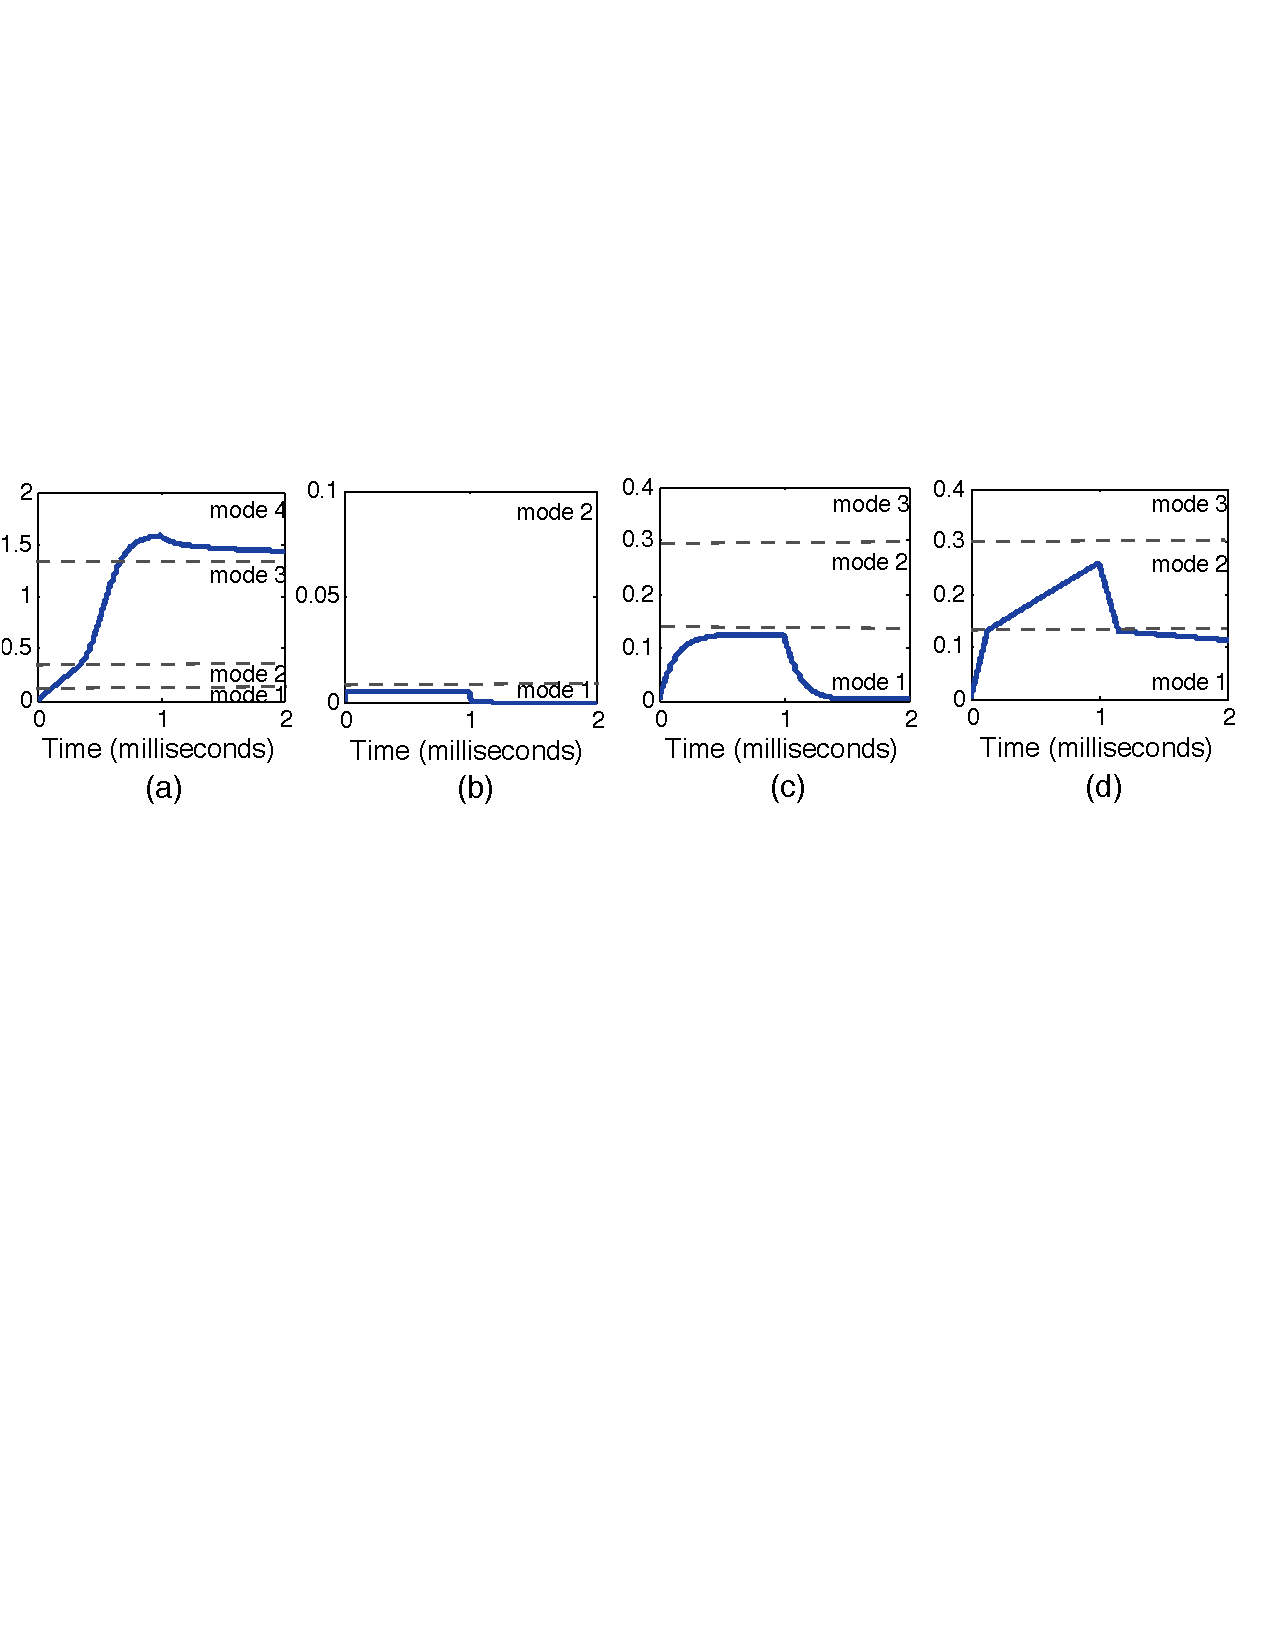
\includegraphics[scale=0.6]{fig-cardiactraj2}
\caption{Simulation results using disease related parameter values. (a) Original parameters (b) $\tau_{o1}=0.0055$ (c) $\tau_{o2} = 0.125$ (d) $\tau_{so1} =1.2$, $\tau_{so2} =1.0$ }
\label{cresults}
 %\vspace{-0.7cm}
\end{figure}

%%% Local Variables:
%%% TeX-master: "main"
%%% End:


\section{Conclusion}
%Hybrid automata are well-studied formalisms for modeling the behavior of biological systems. In this article, we have presented a framework using $\delta$-complete decision procedures for the parameter identification of hybrid biological systems. We have used $\delta$-satisfiable formulas to describe parameterized hybrid automata and to encode parameter synthesis problems. We have employed the $\delta$-decision procedures to perform bounded model checking, and developed an interval constrains propagation based algorithm to obtain the resulting parameters.
We have presented a framework using $\delta$-complete decision procedures for the parameter identification 
of hybrid biological systems. We have used $\delta$-satisfiable formulas to describe parameterized hybrid automata 
and to encode parameter synthesis problems. We have employed $\delta$-decision procedures to perform bounded model 
checking, and developed an algorithm to obtain the resulting parameters.
We have demonstrated the applicability of our method on a highly nonlinear hybrid model of a cardiac cell that cannot
be handled by other verification tools. We have successfully ruled out model candidates which did not fit 
experimental observations, and we have identified critical parameter ranges that can induce cardiac disorders.
Our method has the potential to be applied to model classes such as hybrid functional Petri nets models \citep{hfpn}. 
We plan to explore this in future work. Another interesting direction is applying our method for parameter estimation 
from experimental data. By properly encoding the noisy wet-lab experimental data using logic formulas, bounded model 
checking can be utilized to find the unknown parameter values. In this respect, the parameter 
estimation framework presented in \cite{liu13} promises to offer helpful pointers.

%Finally, we will develop a GPU-based implementation of our method to exploit the inherent massive parallelism in generating trajectories through numerical integration.





%\paragraph{Funding:} This work has been partially supported by the National Science Foundation (NSF), NSF Expeditions in Computing.

%\paragraph{Conflict of Interest:} none declared.


%%% Local Variables:
%%% TeX-master: "main"
%%% End:


\bibliographystyle{abbrv}
\bibliography{ref}

\end{document}

%%% Local Variables:
%%% mode: latex
%%% TeX-master: t
%%% End:
